\section{Analyse eines optimalen DevSecOps Prozesses}\label{sec:analysisDevSecOps}
Was ist DevSecOps?
Warum benötigt man DevSecOps?
Wie sollte DevSecOps aussehen?
Was muss man beachten?

Diese Fragen sollen in der folgenden Analyse Schritt für Schritt beantwortet werden und bilden die Basis für das grundlegende Verständnis von DevSecOps Prozessen.

\subsection{DevOps}
Die Frage, was DevOps eigentlich sei, ist etymologisch leicht zu beantworten.
DevOps ist ein Kofferwort aus den Komponenten "Development" und "Operations".
Die Bedeutung dieses Begriffs hingegen stellt sich als weit weniger eindeutig heraus.
Die Antwort auf die Frage nach der Bedeutung ist vielmehr ein Verständnis für ein Ziel, welches versucht wird zu erreichen, eine Philosophie Prozesse zu optimieren und ein "Ansatz, wie die Zusammenarbeit zwischen Softwareentwicklung und IT-Betrieb verbessert werden kann."\cite{DevOps2021}

Microsoft Azure, einer der führenden Betreiber im DevOps Segment, beschreibt in einem Blogpost diese Philosophie als eine Art Brücke zwischen IT-Betrieb, Qualitätstechnik und Sicherheit\cite{WasIstDevOps}:
\begin{quote}
    DevOps ermöglicht es zuvor getrennten Rollen wie Entwicklung, IT-Betrieb, Qualitätstechnik und Sicherheit, sich zu koordinieren und zusammenarbeiten, um bessere und zuverlässigere Produkte zu liefern.
    Durch die Einführung der DevOps-Kultur mit DevOps-Methoden und -Tools können Teams besser auf die Anforderungen ihrer Kunden reagieren, das Vertrauen in ihre eigenen Anwendungen steigern und Geschäftsziele schneller erreichen.
\end{quote}

Zusammenfassend lässt sich sagen, dass DevOps ein Mindset, eine Philosophie oder ein Prozess ist, der den von Natur aus zyklischen Prozess der Softwareentwicklung automatisieren, koordinieren, strukturieren und beschleunigen soll.
Was zunächst komplex klingt kann heutzutage mithilfe vieler Tools auf dem Markt verhältnismäßig leicht erreicht werden.
Im Laufe des Seminars wurde hierfür primär die Plattform GitLab CI eingesetzt, welche auch hier später als Beispiel dienen wird.
Wichtig ist allerdings ein Verständnis dafür zu entwickeln, dass GitLab nicht die Lösung für DevOps ist, sondern nur ein Tool, wie viele andere auch, um das Mindset eines Entwickler- und Operationsteams elegant umsetzen zu können.

\subsection{Left Shift in DevOps}

Der Begriff "Left Shift" beschreibt den Ansatz Tests so früh wie möglich, also zeitlich weiter links, anzuordnen.
Dadurch entsteht ein erhöhter Fokus auf Tests und somit im Idealfall auch ein höherer Qualitätsstandard bei der Entwicklung der Software.\cite{dr.darrellr.schragDevOpsShiftLeft2016}
Dies geschieht durch das direkte Feedback, welches nun an jeden commit\footnote{Ein commit beschreibt eine Menge an Änderungen, welche vom Entwickler in das Versionskontrollsystem eingefügt werden. Im Fall dieses Seminars ist das Versionskontrollsystem git, bzw. GitLab. Nähere Informationen dazu sind später in Kapitel~\ref{subsec:git-struktur/branching} zu finden.} geknüpft ist.
Somit können Unschönheiten und Fehler direkt behoben werden, ohne dass sie weitere negative Effekte auslösen können.

Dies muss sich nicht ausschließlich auf Unit-/Integration- und End-To-End-Tests beziehen, sondern kann auch auf Security Tests, hier im Speziellen \hyperref[subsubsec:dast]{DAST}, bezogen werden.
Hierbei kann man sogar so weit gehen, dass alle sicherheitsrelevanten Tests nach jedem Commit ausgeführt werden sollten, selbst wenn diese eine hohe Zeit in Anspruch nehmen.
Dies hat den Vorteil, dass Entwickler ein umgehendes Feedback erhalten, über alle Sicherheitslücken, die in dem aktuellen Commit gefunden werden.
Daher wird dies auch von vielen Experten empfohlen, unter welchen auch GitLab ist, deren Tool die Grundlage für die Umsetzung einer Pipeline in diesem Seminar geboten hat.\cite{gitlabSeismicShiftApplication2020}
Dadurch, dass Sicherheitslücken nun gemeinsam mit den Testergebnissen direkt an die Entwickler zurückgegeben werden fließt das Beheben von Sicherheitslücken nahtlos in den Prozess der Behebung von Fehlern und der Entwicklung neuer Features ein.


\subsection{DevSecOps}

Etymologisch lässt sich auch der Begriff DevSecOps schnell erklären.
Das Kofferwort DevOps wurde lediglich um die Komponente der "Security" erweitert.
Die Umsetzung einer guten Integration eines Sicherheitsaspekts in einen DevOps Prozess ist allerdings nicht sehr einfach, da hierbei die Entwicklung ausgebremst werden kann.
Dennoch ist der Sicherheitsaspekt bei einer Software nicht zu unterschätzen und sollte als zentraler Bestandteil einer DevSecOps Pipeline gesehen werden.
IT-Sicherheit ist grundsätzlich ein Wettrennen.
Während einige Entwickler/Security Experten versuchen eine Software zu schützen, versuchen Hacker Schwachstellen zu finden und zu nutzen.
Außerdem ist IT-Sicherheit ein sehr komplexes Thema, welches in nahezu jedem Fall Experten benötigt.

Allerdings lassen sich auch viele Teile der Überprüfung auf Schwachstellen automatisieren und nach links shiften.
Hierfür gibt es verschiedene Punkte und Möglichkeiten, an denen man ansetzen kann.
Einige davon werden später genauer erläutert, weshalb sie hier nur eine kurze Erwähnung finden sollen.
Ein wichtiger Bestandteil bei der Umsetzung einer DevSecOps Pipeline ist ein guter Feedbackloop zwischen Entwicklern und Sicherheitsexperten, die helfen können gefundene Sicherheitslücken einzuordnen und falls nötig zu beheben.
Dies kann beispielsweise durch automatische Issues erreicht werden, die von den entsprechenden Schritten angelegt werden und den Entwicklern und Sicherheitsexperten die Möglichkeit geben über vorhandene Lücken zu diskutieren.
GitLab bietet hierfür die Möglichkeit bei gefundenen Sicherheitslücken im \hyperref[subsubsec:dast]{DAST} oder bei der Verwendung des integrierten \hyperref[subsubsec:vulChecker]{Vulnerability Checkers} mit einem Klick ein Issue für eine Sicherheitslücke in den integrierten GitLab Issue Boards anzulegen.
Wie genau dieser Loop insgesamt aussehen kann und sollte wird später noch graphisch visualisert (Siehe Abbildung~\ref{fig:devSecOpsProcess}).

\subsection{Entwicklungsprinzipien}

Der Bereich der agilen Entwicklung hat in den letzten Jahren viele verschiedene Verfahren entwickelt, um Projekte zu managen und agil zu arbeiten.
"Agile Softwareentwicklung zeichnet sich durch selbstorganisierende Teams sowie eine iterative und inkrementelle Vorgehensweise aus."\cite{AgileSoftwareentwicklung2021}
Der Kern agiler Softwareentwicklung ist also, das Kurzhalten von Planungsphasen und damit einhergehender kontinuierlicher weiterer Planung zur Laufzeit des Projekts.
Ähnlich wie bei DevOps ist das Ziel, sich möglichst schnell und flexibel auf Änderungen anpassen zu können, kontinuierlich neuen Code vorweisen können und sich "in regelmäßigen, kurzen Abständen mit dem Kunden [abstimmen]"\cite{AgileSoftwareentwicklung2021} zu können und dabei die Codequalität zusätzlich positiv zu beeinflussen.
Hier greifen DevOps und agile Methoden Hand in Hand.
Agile Methoden können sehr schnell sehr komplex werden, weshalb sie in dieser Arbeit nur so weit beschrieben werden, dass der Zusammenhang zur DevSecOps Philosophie offensichtlich werden.
Daher soll hier ein grundlegendes Verständnis für Kanban und Scrum gegeben werden, da agile Entwicklung eine wichtige Voraussetzung für ein gutes und erfolgreiches DevOps orientiertes Projekt ist.

\subsubsection{Kanban}\label{subsubsec:kanban}

Wie bei vielen agilen Methoden steht im Zentrum von Kanban ein Board für die visualisierung einzelner Arbeitsschritte.
Auf diesem sind alle zu tätigen Aufgaben eingetragen, welche Schritt für Schritt in Bearbeitung gehen können.
Zur Unterscheidung dieser Zustände führt man mehrere, aber mindestens drei, Spalten ein.
Diese sind meist mit den Begriffen "Backlog", "In Progress" und "Completed" gekennzeichnet.
Im Backlog befinden sich alle noch nicht begonnenen Aufgaben, die bei Bedarf in Bearbeitung gehen können.
In diesem Fall wird die Karte aus der Spalte "Backlog" in die Spalte "In Progress" bewegt, um für alle Mitarbeitenden zu signalisieren, dass an dieser Aufgabe bereits gearbeitet wird.
Nach Fertigstellung einer dieser Karten wird diese in die Spalte "Completed" verschoben und ist damit erledigt.
Um verschiedene Wichtigkeitsstufen abbilden zu können ist möglich verschiedene sog. Lanes zu verwenden.
Diese werden als einzelne Reihen dargestellt, von denen in der Regel obere Reihen vor unteren Reihen bearbeitet werden sollen.
Zudem limitiert man die Anzahl maximal erlaubter Aufgaben in Bearbeitung, um zu starkes Multitasking und damit einhergehender sinkender Effizienz zu vermeiden.

Positiv lässt sich hier anmerken, dass durch ein sehr offenes, transparentes Prinzip ein gleichmäßiger Workflow entsteht, der sich in den meisten Situationen einfach in bestehende Prozesse integrieren lässt.

Dem entgegen steht ein Problem, welches dadurch entsteht, dass keinerlei Möglichkeiten zur Zeitplanung in Kanban vorgesehen sind.
Dies kann dazu führen, dass Deadlines nicht eingehalten werden können, da sich Entwickler oder Manager leichter in der Aufgabenverteilung verschätzen.
Zudem ist es bei Kanban nötig, alle vorhandenen Aufgaben in einzelne unabhängige Schritte aufteilen zu können.
Dies kann allerdings nicht immer gewährleistet werden, sollte in der Softwareentwicklung allerdings meistens kein Problem sein, da grundsätzlich Abstraktion in kleine Pakete in jeder Codebasis wünschenswert ist.\cite{Kanban}

\subsubsection{Scrum}

Atlassian, zieht bei der Beschreibung von Scrum eine sehr passende Football Analogie heran\cite{atlassianScrumWasEs}:
\begin{quote}
    Scrum ist ein Framework, das die Zusammenarbeit in Teams unterstützt. \textit{Scrum} steht im Rugby für \textit{Gedränge} – und genau wie ein Rugbyteam, das für das große Spiel trainiert, sind Teams mit Scrum in der Lage, durch Erfahrungen zu lernen, sich bei der Problembehebung selbst zu organisieren sowie ihre Erfolge und Niederlagen zu reflektieren, um sich kontinuierlich zu verbessern.
\end{quote}

Ähnlich wie bei \hyperref[subsubsec:kanban]{Kanban} werden Aufgaben aufgeteilt in "Backlog", "In Progress" und "Completed".
Allerdings liegt ein weitaus größerer Fokus auf der Zeitplanung, die bei \hyperref[subsubsec:kanban]{Kanban} außer Acht gelassen wird.
Im Gegensatz zu Kanban werden die Aufgaben nicht einfach bearbeitet, sobald die vorherige Aufgabe abgeschlossen wird, sondern es wird für einen kurzen Zeitraum, meist zwei Wochen, geplant, welche Aufgaben zu erledigen sind.
Dieser Zeitraum nennt sich Sprint und stellt die Basis von Scrum dar.
In regelmäßigen Meetings legt ein sog.\ Scrum Master die einzelnen Aufgaben fest, die im nächsten Sprint erledigt werden sollen und weist diese oftmals direkt Mitarbeitern zu, die diese Aufgaben im Laufe des Sprints erledigen sollen.

Dies sorgt für eine enorm hohe Struktur und ein außerordentliches Zeitmanagement, welches in Kanban so nicht gewährleistet werden kann.
Allerdings sind zweiwöchige (einmal pro Sprint) Besprechungen oftmals nicht flexibel genug, um schnellen Entscheidungen eines Kunden zu entsprechen, was zu Planungsschwierigkeiten führen kann.

\subsubsection{Fazit}

Die beiden oben genannten Methoden bieten eine gute Grundlage für DevSecOps.
Insgesamt muss jedes Team für sich entscheiden, welches Entwicklungsprinzip für sie am besten funktioniert.
Alle Prinzipien einmal auszuprobieren ist definitiv empfehlenswert, um den optimalen Workflow für sein Team und seine Anwendungsfälle finden zu können.

\subsection{Git Struktur/Branching}\label{subsec:git-struktur/branching}

Bevor eine Betrachtung der einzelnen Schritte im Prozess stattfinden kann, muss zunächst die Grundstruktur des Versionskontrollsystems (VCS) geklärt sein.
In diesem Seminar wurde als VCS GitLab (git) verwendet, weshalb dieses auch hier als Grundlage dienen soll.
Wenn es um das Thema Struktur im git geht, entstehen häufig hitzige Diskussionen unter Entwicklern.
Die Menge an möglichen Modellen ist scheinbar endlos.
In der Vergangenheit hat sich oft gezeigt, dass git-flow\cite{SuccessfulGitBranching} eine gute Möglichkeit ist, um sein git zu ordnen.
Allerdings ist dieses Modell sehr kompliziert, weshalb von diesem Modell heutzutage oftmals abgeraten wird.
Ein häufig vorgeschlagenes Alternativmodell stellt GitHub flow\cite{UnderstandingGitHubFlow} dar.
Dieses Modell ist im Gegensatz zu git-flow sehr einfach gestrickt.
So einfach, dass Testumgebungen nicht wirklich anhand der gegebenen Branches dargestellt werden können.
Deshalb empfiehlt sich die Verwendung eines Modells, das zwischen git-flow und GitHub flow anzuordnen ist.
\begin{figure}[H]
    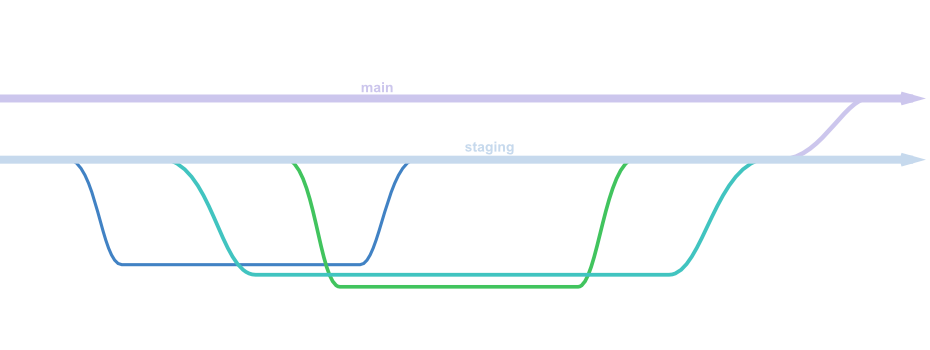
\includegraphics[width=0.8\textwidth]{img/branching}
    \centering
    \caption{Graphische Darstellung der Kombination aus git-flow und GitHub Flow}
    \label{fig:branchingModel}
\end{figure}

Das hier gezeigte Modell basiert relativ stark auf GitHub flow.
Es gibt einen Hauptbranch (Main), welcher zu jeder Zeit veröffentlichbar sein sollte.
Im Gegensatz zu GitHub flow ist dies allerdings nicht der main Branch, sondern ein staging Branch.
Dieser kann dann Nutzern als Beta-Version zur Verfügung gestellt werden.
So haben Nutzer die Möglichkeit neue Features sofort zu testen und direktes Feedback in den Entwicklungsprozess zurück zu bringen.
Im Gegensatz zu GitHub flow ist dies allerdings nicht der Branch, der in Production veröffentlicht wird.
Dafür gibt es den main branch, für den die gleichen Kriterien gelten wie für den Staging Branch.
Zudem darf auf den main branch allerdings nur eine getestete Version vom Staging Branch deployed werden.
Entwicklung sollte allerdings, genau wie bei GitHub flow, auf dem Main und Staging branch nicht stattfinden.
Hierfür werden für jedes Feature eigene Branches aufgemacht (dunkelblau, hellblau und grün in Abbildung~\ref{fig:branchingModel}).
Auf diesen werden alle commits gepushed, bis das feature bereit ist, in den Staging branch gemerged zu werden.
Dies bedeutet, dass das Feature vollständig funktioniert.
Sobald dieses Stadium erreicht ist, wird ein Pull Request in den Staging Branch erstellt.
Hiermit wird der Review Prozess eingeleitet.
Zunächst laufen natürlich alle automatisierten Tests und stellen die Codequalität und -funktionalität bestmöglich fest.
Im nächsten Schritt sollte der Merge Request von anderen Personen bestätigt werden und mögliche Fehler und Unstimmigkeiten sollten behoben werden.
Sobald diese Schritte durchlaufen sind, kann das Feature in den Staging Branch gemerged werden.
Nun rollt die Pipeline das Feature automatisch an alle Beta Nutzer aus, sodass eine realistische Testumgebung Feedback in den Entwicklungsprozess zurückspielen kann.
Unter der Annahme, dass hierbei keine Fehler auftreten kann man nun mit erhöhter Sicherheit und Stabilität den Staging Branch nach einem Pull Request in den Main Branch mergen, was ein Deployemnt für alle Nutzer auslöst.

Die Vorteile gegenüber GitHub flow liegen auf der Hand.
Ein Branchingmodell, welches nur minimal komplizierter ist, bringt eine stark erhöhte Stabilität im Programm, da Features zunächst an eine kleine Testgruppe ausgerollt wird, Feedback gesammelt wird und dieses erneut in den Entwicklungsprozess einfließen kann, bevor ein Feature an alle Nutzer ausgerollt wird.
Alle Vorteile von GitHub Flow gegenüber git-flow bleiben allerdings erhalten, weshalb dies immer noch ein exzellentes Modell für DevOps ist.

\subsection{DevSecOps Pipelines}

Pipelines bilden die Grundlage in der Umsetzung eines erfolgreichen DevSecOps Projekts.
Grundsätzlich lassen sich Pipelines in drei Bereiche unterteilen: Testen, Bauen und Deployen.
Allerdings lassen sich diese Schritte nicht immer einfach nacheinander ausführen, da Schritte im Test beispielsweise von einem Build oder Deployment abhängen können, genauso wie ein Deployment von einem Test und offensichtlich einem Build abhängen kann.
Daher werden einige der wichtigsten Schritte im Folgenden nacheinander einzeln betrachtet und analysiert.
Aufgrund der teils hohen Komplexität einiger Schritte werden alle einzelnen Schritte nur angeschnitten, um einen Überblick über die nötigen Funktionen einer guten Pipeline zu erhalten.
Diese sind chronologisch so angeordnet, wie sie auch im finalen Prozess vorhanden sein sollten.

\subsubsection{Coding Richtlinien/Code Architektur}\label{subsubsec:codingguidelines/codearchitecture}

Nachdem nun klar ist, in welcher Struktur der Code im VCS vorzufinden ist, gilt es nun die einzelnen Schritte in der Pipeline zu betrachten.
Hierbei sollte mit den Syntax- und Architekturtests begonnen werden.
Bevor die Funktionalität einer Software getestet wird, sollte immer sichergestellt sein, dass die Architektur und Syntax den gewählten Konventionen entspricht.
Für die Bewertung der Position eines Schrittes in einer Pipeline gibt es mehrere ausschlaggebenden Punkte, welche bei jedem Job in der Pipeline betrachtet werden sollten.
\begin{itemize}
    \item Welche Abhängigkeiten existieren zu anderen Schritten in der Pipeline?
    \item Wie hoch ist die Zeitkomplexität des Jobs?
    \item Wann in der Pipeline muss dieser Job ausgeführt werden?
\end{itemize}

\paragraph{Welche Abhängigkeiten existieren zu anderen Schritten?}

Bei der Betrachtung der Abhängigkeiten zu anderen Schritten liegt auf der Hand, dass nichts außer dem Source Code nötig ist, um dessen Qualität zu testen.
Somit gibt es keine anderen Jobs, welche vor diesem Job auszuführen sind.
Dies ist auch der Grund, weshalb dieser Schritt zu Beginn der Pipeline angeordnet sein sollte.

Da auch keine anderen Tests Abhängigkeiten zu Architektur- und Syntaxtests haben lassen sich diese auch problemfrei zu anderen Tests parallelisieren.

\paragraph{Wie hoch ist die Zeitkomplexität des Jobs?}

Syntax- und Architekturtests sind in relativ kurzer Zeit auszuführen, da keine externen Abhängigkeiten oder komplexe Build Prozesse nötig sind.
Dies ist speziell in den ersten Jobs äußerst erstrebenswert, da die Pipeline möglichst früh fehlschlagen sollte, wenn Fehler existieren, um unnötige Verzögerungen im Entwicklungsprozess zu vermeiden.
Zudem ist auch die Behebung von Syntaxfehlern zumeist relativ schnell erledigt, sodass zügig die weiteren Schritte der Pipeline erreicht werden können.

\paragraph{Wann muss dieser Job ausgeführt werden?}

Bei dieser Frage ist die Zeitkomplexität oftmals ein großer Faktor.
Tests, die kaum Zeit in Anspruch nehmen kann man ohne große Einschränkungen häufiger ausführen.
Dementsprechend empfiehlt es sich hier, die Tests bei jedem commit auszuführen, um stets eine gute Codequalität gewährleisten zu können und bereits früh im Prozess korrigieren zu können, falls die Architektur nicht den gesetzten Standards entspricht.

\subsubsection{Vulnerability Checker}\label{subsubsec:vulChecker}

Bei der Entwicklung großer Projekte ist es kaum möglich externe Abhängigkeiten zu vermeiden.
Für nahezu jedes Framework und jede Programmiersprache existieren Package Manager, die den Prozess externe Pakete ins Projekt einzufügen extrem vereinfachen.
Diese Leichtigkeit löst allerdings ein Problem aus.
Viele Libraries wurden selbst von unerfahrenen Entwicklern geschrieben, oder wurden in sehr kurzer Zeit entwickelt, was zu Fehlern und vor allem zu Sicherheitslücken führen kann.
Die Entwicklercommunity kann diese zwar häufig relativ schnell finden und identifizieren, aber Maintainer können die Sicherheitslücken oftmals nicht sofort schließen.
Daher ist ein wichtiger Faktor einer guten Pipeline Abhängigkeiten auf bekannte Lücken zu prüfen.
Hierfür gibt es Datenbanken, die von der Community gepflegt werden und mit nahezu allen bekannten Sicherheitslücken gefüllt sind.
In diesem Job in der Pipeline geht es also darum, die Quelldateien, zumeist Abhängigkeitsdateien der Paketmanager (z.B. package.json oder requirements.txt), gegen diese Datenbanken zu prüfen und den Entwicklern Feedback zu geben, falls bekannte Sicherheitslücken existieren.

\paragraph{Welche Abhängigkeiten existieren zu anderen Schritten?}

Auch hier lässt sich feststellen, dass keine Abhängigkeiten zu anderen Schritten in der Pipeline existieren.
Lediglich zum Source Code (wobei möglicherweise sogar einzelne Dateien reichen, wie zum Beispiel package.json oder requirements.txt) und zu den Vulnerability Datenbanken existieren externe Abhängigkeiten.
Deshalb lässt sich dieser Schritt zusammen mit den vorher genannten parallel ausführen.

\paragraph{Wie hoch ist die Zeitkomplexität des Jobs?}

Die Zeitkomplexität ist relativ gering, wenn man einen der gängigen Paketmanager verwendet. (z.B.\ npm, pip)
Viele Tools zur Bewertung von Paketen verwenden eine Datenbank, in der sie sehr schnell überprüfen können, ob für die angegebene Version Sicherheitslücken gemeldet sind.

\paragraph{Wann muss dieser Job ausgeführt werden?}

Wie bereits zuvor ist die geringe Zeitkomplexität ein Grund, weshalb sich dieser Schritt gut häufig ausführen lässt.
Zudem existieren keine weiteren Abhängigkeiten, weshalb der Job auch gut parallel ausgeführt werden kann.
Selbst, wenn dies aber nicht der Fall wäre sollte man diese Stufe dennoch bei jedem Commit ausführen und überprüfen, ob neu hinzugekommene Pakete bekannte Schwachstellen enthalten.
Allerdings ist dies leider noch nicht vollständig ausreichend, da Sicherheitslücken auch später entdeckt werden können.
Daher empfiehlt es sich, diese Tests je nach aktuellem Entwicklungsstand und der Häufigkeit von commits in einem Scheduled Lauf der Pipeline ebenfalls durchzuführen, um neue Sicherheitslücken möglichst schnell zu finden, auch wenn an dem Projekt nicht mehr aktiv entwickelt wird.

\subsubsection{Lizenzüberprüfung}

Die Aufgabe der Lizenzüberprüfung scheint zunächst simpel und einleuchtend, stellt sich aber bei näherer Betrachtung als überraschend komplex dar.
Die Komplexität vieler Lizenzen macht es Entwicklern oft nicht leicht zu entscheiden, welche Pakete problemfrei verwendet werden dürfen oder nicht.
Oftmals werden auch Abhängigkeiten von Abhängigkeiten, etc. zum Problem.
Hierbei eine gute Übersicht zu behalten ist ohne dem richtigen Tooling nahezu unmöglich.
Außerdem liegt die Entscheidung der erlaubten Lizenzen oftmals nicht in der Hand der Entwickler, sondern einer gezielten Rechtsabteilung.
Mithilfe einer guten Lizenzprüfung kann man hier also eine Brücke schlagen für eine nahtlose Kooperation zwischen Entwicklern und rechtlichen Lizenzaspekten, ohne dass Entwickler einen tiefen Einblick in Lizensierungsmodelle benötigen und ohne, dass die Rechtsabteilung irgendwelche Informationen über Softwareentwicklung benötigt, um eine korrekte Lizenzierung validieren zu können.

\paragraph{Welche Abhängigkeiten existieren zu anderen Schritten?}

Da die Lizenzüberprüfung lediglich Informationen über die eingebundenen Pakete benötigt, wie auch zuvor schon bei dem Vulnerability Checker verhält es sich auch bei den Abhängigkeiten genau gleich.
Außer einer äußeren Abhängigkeit zu den entsprechenden Paketquellen gibt es keine weiteren Abhängigkeiten, im Speziellen nicht zu anderen Schritten in der Pipeline.
Daher lässt sich auch dieser Job problemfrei zu Beginn der Pipeline parallel zu den vorhergegangen Schritten ausführen.

\paragraph{Wie hoch ist die Zeitkomplexität des Jobs?}

Da hierbei lediglich Lizenzen gegen Regeln geprüft werden müssen, ist dieser Job sehr schnell ausführbar, besonders, wenn nur neue oder aktualisierte Lizenzen geprüft werden.

\paragraph{Wann muss dieser Job ausgeführt werden?}

Da ein Paket in einer festen Version seine Lizenzierung nicht einfach ändern kann, reicht es völlig aus bei jedem commit zu prüfen, ob sich Pakete verändert haben.
Sobald eine Veränderung in den verwendeten Paketen zu finden ist, sollte die Pipeline die Lizenzen der entsprechenden Lizenzen überprüfen.

\subsubsection{Dynamic Application Security Testing (DAST)}\label{subsubsec:dast}

Dynamic Application Security Testing beschreibt den Prozess eine laufende Anwendung mit einem Black Box Verfahren aktiv auf Sicherheitslücken zu überprüfen.
Black Box Verfahren bedeutet, dass keinerlei interne Informationen wie zum Beispiel Secrets oder Source Code für die Überprüfung zur Verfügung stehen.
Dies stellt daher das realistischste aller möglichen automatisierten Testverfahren dar.
Die \textit{aktive} Überprüfung auf Sicherheitslücken bedeutet, dass tatsächlich mit dem Ziel die Anwendung von außen zu zerstören, oder Daten zu manipulieren vorgegangen wird.
Daher sollten diese Tests niemals auf einer produktiven Umgebung ausgeführt werden.
Dennoch sollen die Ergebnisse der Tests repräsentativ für ein Echtweltszenario sein.
Daher empfielt es sich, eine Testumgebung zu verwenden, die nahezu identisch zur Produktivumgebung aufgesetzt ist.
Docker bietet hier vor allem in Kombination mit GitLab CI eine sehr gute Möglichkeit dies zu erreichen, wie im \hyperref[sec:gitlab-ci-im-einsatz-als-dast-tool]{letzten Kapitel} näher beschrieben wird.

\paragraph{Welche Abhängigkeiten existieren zu anderen Schritten?}

Da dieser Schritt eine fertige Anwendung testen soll, ist dieser stark Abhängig von allen Schritten, die nötig sind, um die Anwendung zu bauen und zu deployen.
Diese lassen sich nur sehr schwer generalisieren, da jede Anwendung unterschiedliche Buildprozesse hat.
Dennoch wird DAST aufgrund der starken Abhängigkeit meist als letzter Schritt in der Pipeline ausgeführt.

\paragraph{Wie hoch ist die Zeitkomplexität des Jobs?}

Die Zeitkomplexität von DAST ist enorm hoch.
Dies hängt mit der Komplexität und der Verlangsamung von Test durch die interaktion mit graphischen Bedienelementen zusammen.
Bei DAST werden Websiten zunächst nach allen möglichen Routen der Anwendung abgesucht.
Dazu wird ein Crawler verwendet welcher Schritt für Schritt versucht alle Links, Buttons und Eingabefelder zu bedienen um im Idealfall alle erreichbaren Routen zu finden.
Je nach Komplexität der Anwendung kann dies allein bereits bis zu 30 Minuten dauern.
Sobald alle zu Testenden Seiten gefunden sind werden die gewünschten Sicherheitslücken auf der Website gesucht.
Hierzu wird versucht mit gezielten Eingaben ein Fehlverhalten auszulösen.
Da dies viele Schritte und Versuche mit sich bringt, kann die Dauer einer DAST Stage bis zu mehreren Stunden an Zeit in Anspruch nehmen.
Somit ist nicht nur die starke Abhängigkeit, sondern auch die hohe Zeitkomplexität des Jobs ein Grund dafür ihn am Ende der Pipeline auszuführen.

\paragraph{Wann muss dieser Job ausgeführt werden?}

Hierbei gibt es viele verschiedene Auffassungen.
Mindestens aber vor jeder Veröffentlichung sollte die Pipeline laufen, um gewährleisten zu können, dass die gröbsten Sicherheitslücken gefunden wurden.
Desto öfter die Pipeline ausgeführt wird desto schneller können Sicherheitslücken behoben werden und desto direkter ist das Feedback an die Entwickler.
Dies ist grundsätzlich empfehlens- und wünschenswert.
Deshalb wir auch oft, zum Beispiel auch von GitLab empfohlen, die Pipeline bei jedem Commit laufen zu lassen.\cite{gitlabSeismicShiftApplication2020}
Dem entgegen steht die hohe Zeitkomplexität und die damit verbundene Auslastung der Serverinfrastruktur.
Daher muss jedes Entwicklerteam selbst abwägen, wie oft dieser Schritt durchgeführt werden sollte.


\subsubsection{Visualisierung eines optimalen DevSecOps Prozesses}
\begin{figure}[H]
    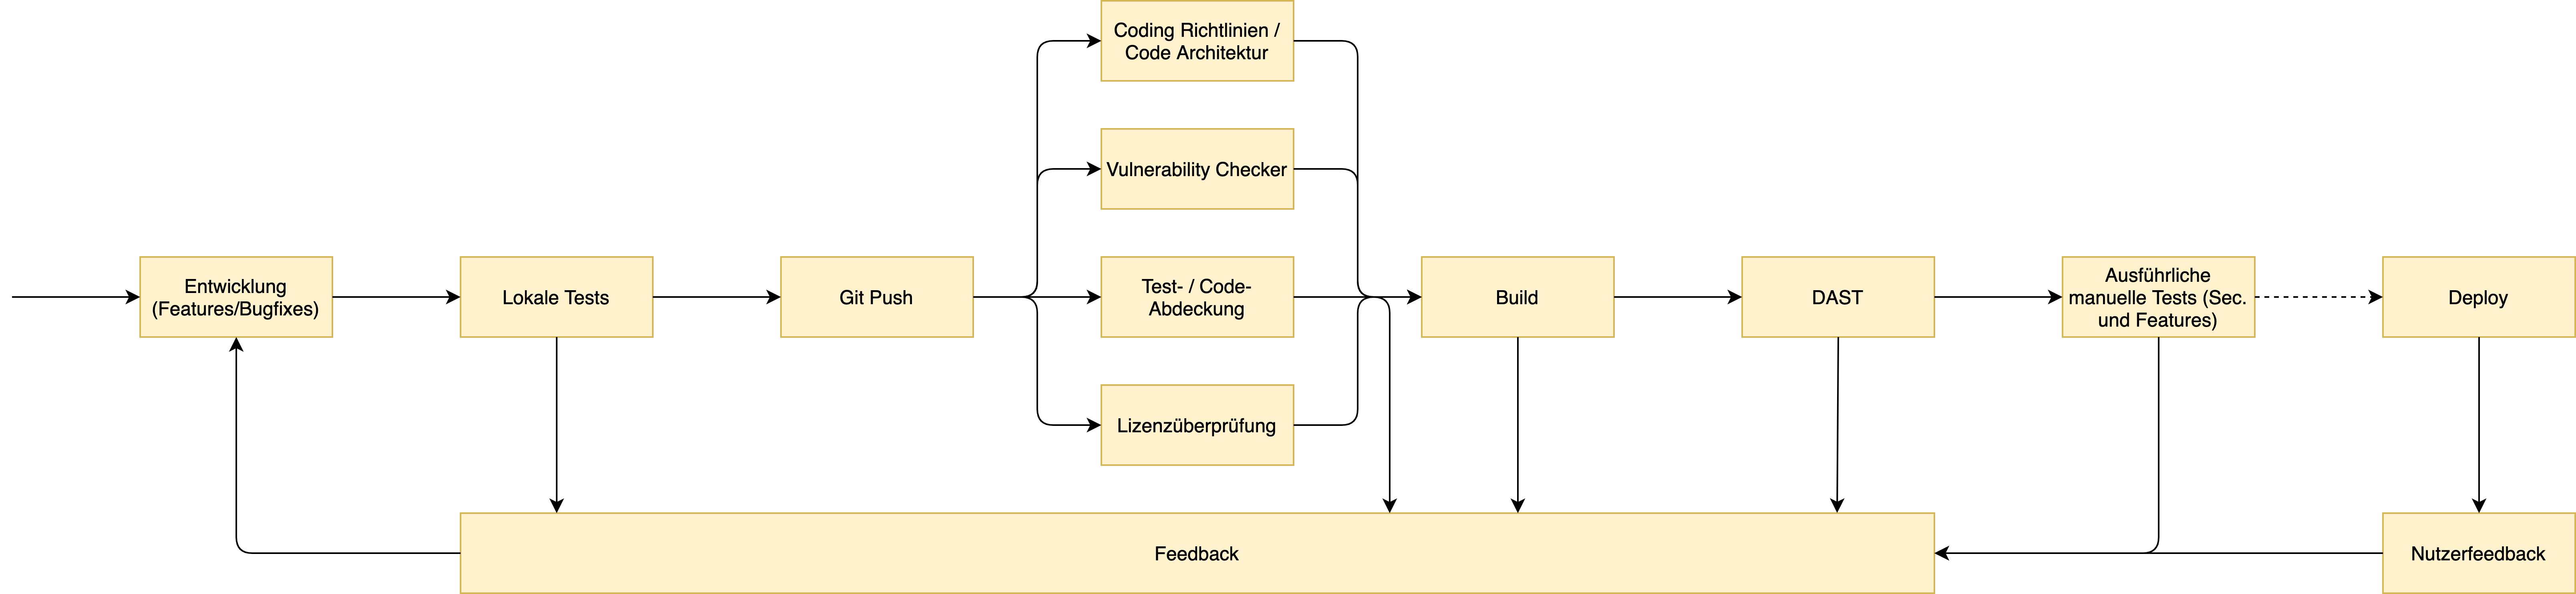
\includegraphics[width=0.8\textwidth]{img/DevOpsWorkflow}
    \centering
    \caption{Graphische Darstellung eines optimalen DevSecOps Prozesses}
    \label{fig:devSecOpsProcess}
\end{figure}